\RequirePackage[T1]{fontenc}
\documentclass[conference]{IEEEtran}
\usepackage{amsmath}
\usepackage{graphicx}
\usepackage{booktabs}
\usepackage{url}
%% Generated from verified results. Do not hand-edit.
\newcommand{\LogAcc}{84.520}
\newcommand{\LogFone}{84.412}
\newcommand{\LogTime}{5.39}
\newcommand{\PlainAcc}{90.980}
\newcommand{\PlainAccSD}{0.046}
\newcommand{\PlainFone}{90.927}
\newcommand{\PlainFoneSD}{0.017}
\newcommand{\PlainTime}{62.55}
\newcommand{\PlainTimeSD}{10.09}
\newcommand{\DropAcc}{90.793}
\newcommand{\DropAccSD}{0.153}
\newcommand{\DropFone}{90.706}
\newcommand{\DropFoneSD}{0.146}
\newcommand{\DropTime}{77.43}
\newcommand{\DropTimeSD}{11.33}
\newcommand{\MeanDelta}{-0.221}
\newcommand{\NeuralGain}{6.515}
\newcommand{\BaselineBudget}{23.85}
\newcommand{\BaselineAllBudget}{42.21}
\newcommand{\NormMean}{0.28588690}
\newcommand{\NormSD}{0.35293528}
\newcommand{\CheckInitialLoss}{2.32058}
\newcommand{\CheckFinalLoss}{0.000649}
\newcommand{\CNNParams}{105,866}
\newcommand{\LogParams}{7,850}
\newcommand{\TotalCNNTime}{419.93}

\graphicspath{{../figures/}}
\title{Does Head Dropout Help a Small CNN?\\A Controlled Fashion-MNIST Study}
\author{\IEEEauthorblockA{ROBT407: Machine Learning with Applications\\Nazarbayev University\\Team names and individual contributions pending completion}}
\begin{document}
\maketitle
\begin{abstract}
This study tests whether adding dropout to the classification head of a small convolutional neural network improves clothing classification. We preserve Fashion-MNIST's official 10,000-image test set, create one stratified 48,000/12,000 training/validation split, and compare logistic regression with two otherwise identical PyTorch CNNs. The controlled change is head dropout with probability 0.30, specified before training. Both CNNs use the same three seeds, initial weights, minibatch orders, optimizer, 12-epoch budget, and validation checkpoint rule. Logistic regression obtains \LogFone\% test macro-F1. The CNN obtains \PlainFone\,$\pm$\,\PlainFoneSD\%, versus \DropFone\,$\pm$\,\DropFoneSD\% with dropout (mean and sample standard deviation across seeds). Dropout reduces macro-F1 in every matched seed; its mean effect is \MeanDelta\ percentage points. The hypothesis is therefore unsupported under this fixed procedure. Shirts remain the most difficult category, with prominent confusion among shirts, T-shirts, pullovers, and coats. Saved predictions, checkpoints, and an executed notebook reproduce the reported comparison.
\end{abstract}
\begin{IEEEkeywords}
Fashion-MNIST, clothing classification, convolutional neural network, dropout, controlled comparison
\end{IEEEkeywords}

\section{Introduction and Hypothesis}
Classifying clothing images provides a compact setting for studying how a learned image representation differs from a linear pixel classifier. Fashion-MNIST contains small grayscale product images with visually overlapping garment categories~\cite{fashion,dataset}. This project investigates one regularization decision while holding the remaining neural pipeline fixed.

The research question is: \emph{Does adding dropout to the classification head of a small CNN improve macro-F1 on unseen clothing images, and which clothing categories remain hardest to distinguish?} Here, ``unseen'' means the retained official Fashion-MNIST test examples. It does not imply photographs from arbitrary cameras or clothing retailers.

The notebook records the prediction before fitting: dropout with probability $p=0.30$ will improve mean test macro-F1 by discouraging co-adaptation of the head's hidden features and reducing sensitivity to training-specific detail. This rationale follows the original dropout motivation~\cite{dropout}. A moderate rate was prescribed rather than chosen by test performance. The prediction also acknowledges that a compact network and a sizeable training set may leave little overfitting to correct, and that dropout can impede fitting within a fixed training budget.

Directional support requires a positive mean paired macro-F1 difference. Inconsistent seed signs would weaken that support; a negative effect is a valid outcome. The analysis reports every seed, rather than selecting the best test run. Three seeds characterize training variability on one fixed split and test set; they are not three independent population samples or a statistical significance test.

\section{Dataset and Evaluation Design}
\subsection{Provenance, target, and inclusion rules}
We use the original 2017 Fashion-MNIST IDX release from Xiao, Rasul, and Vollgraf~\cite{fashion,dataset}. The local downloader retrieves the authors' four compressed image/label files and verifies the original MD5 values before parsing the binary records. Checksums in \texttt{src/data.py} and \texttt{results/data\_audit.json} identify the exact bytes even if the repository branch changes. The README documents download commands; raw public data are not included in the code ZIP.

Each input is a $28\times28$ grayscale image with unsigned 8-bit pixels in $[0,255]$. The target is one of ten integer class labels, listed with class performance in Table~\ref{tab:classes}. All categories are included. The original development pool has 60,000 images and the official test set has 10,000. Parsing and content checks found no missing pixels or labels. Each class contributes 6,000 development and 1,000 test images.

Before comparing models, the inclusion policy was fixed as follows: preserve the complete official test set; hash raw image pixels using SHA-256; exclude development images whose exact hash appears in test; exclude development hash groups with conflicting labels; retain the lowest original index in each remaining duplicate group. Then split the retained development examples. This policy prevents exact duplicates from crossing development partitions or leaking from test into training. The audit found \emph{zero} duplicate excess images within either original partition, zero shared train/test hashes, and zero conflicting-label development groups. Thus no examples were removed. No original samples were excluded.

\begin{table}[t]
\caption{Fixed partitions and permitted use. Every class is balanced.}
\label{tab:partitions}
\centering
\begin{tabular}{lrrl}
\toprule Partition & Images & Per class & Use \\
\midrule Training & 48,000 & 4,800 & Fit weights/scaler \\
Validation & 12,000 & 1,200 & Select $C$/checkpoint \\
Official test & 10,000 & 1,000 & Frozen evaluation \\
\bottomrule
\end{tabular}
\end{table}

No object, person, or acquisition-group identifier is provided to this pipeline. Exact pixel hashing cannot rule out near duplicates or multiple views of the same item. Consequently, the study claims protection against exact-image leakage, not complete independence of all underlying products.

\subsection{Fixed split and training-only preprocessing}
A stratified 80/20 split of the original training pool uses split seed 407 (Table~\ref{tab:partitions}). Original indices are saved in \texttt{split\_indices.npz}; every model and seed uses them unchanged. Development seeds do not redraw the partitions.

Pixels are converted to floating point and normalized by
\begin{equation}
 z=\frac{x/255-\mu_{\mathrm{train}}}{\sigma_{\mathrm{train}}},
\end{equation}
where the global training-pixel mean is \NormMean\ and standard deviation is \NormSD. Both statistics are fitted using only the 48,000 training images. Validation and test images receive these same constants. This scalar transformation is shared by all models; no imputation, feature selection, augmentation, or additional learned preprocessing is used. Logistic regression flattens the resulting image, while the CNN retains its spatial layout.

\subsection{Metrics and separation of decisions}
The primary metric is macro-F1,
\begin{equation}
 F_{\mathrm{macro}}=\frac{1}{10}\sum_{k=0}^{9}
 \frac{2\,\mathrm{TP}_k}{2\,\mathrm{TP}_k+\mathrm{FP}_k+\mathrm{FN}_k},
\end{equation}
which gives equal weight to every clothing category. Accuracy is the fraction of correctly classified images. Balanced accuracy, the mean per-class recall, is also saved; because test supports are equal, it equals ordinary accuracy here. Reporting it is redundant for this balanced test set but confirms that imbalance is not hiding the comparison.

Validation macro-F1 controls baseline regularization and CNN checkpoint selection. The test set is never used for either decision. After all fits finish, \texttt{frozen\_protocol.json} records the configuration, selected models, timestamp, and SHA-256 hashes of the source files, split, and checkpoints. The evaluation routine checks those hashes before producing any test metric. All seven models then predict the same official indices. Test error inspection is explicitly exploratory and does not alter the frozen models.

\section{Models and Implementation}
\subsection{Classical baseline}
The baseline is multinomial logistic regression with L2 regularization, implemented using scikit-learn~\cite{sklearn}. It receives 784 flattened normalized pixels and learns ten sets of coefficients and intercepts: $10(784+1)=\LogParams$ parameters. It is a credible low-cost baseline because it can learn class-specific pixel patterns, while its linear decision functions cannot represent the CNN's learned local nonlinear features.

We compare $C\in\{0.01,0.1,1\}$, where smaller $C$ means stronger regularization, using the same validation partition. The solver is L-BFGS with tolerance $10^{-4}$. An initial cap of 500 iterations caused the $C=0.1$ and $C=1$ candidates to stop without convergence. Before any CNN run or test evaluation, all three candidates were rerun with a common 5,000-iteration cap. This convergence repair is preserved in \texttt{development\_log.json}; it did not expand the candidate grid. All final candidates converged (Table~\ref{tab:baseline}). Validation selects $C=0.01$, and that training-only fit is retained without refitting on validation.

\begin{table}[t]
\caption{Final baseline search on validation data. All candidates converged. Times exclude the initial convergence-repair attempt.}
\label{tab:baseline}
\centering
\begin{tabular}{rrrr}
\toprule $C$ & Iterations & Macro-F1 (\%) & Fit time (s) \\
\midrule
\csname @@input\endcsname generated/baseline_rows.tex 
\bottomrule
\end{tabular}
\end{table}

\subsection{Small CNN and tensor dimensions}
The CNN is trained from random initialization in PyTorch. Two convolution/ReLU/pooling blocks learn spatial features, followed by a compact classification head. Both convolutions use $3\times3$ kernels, stride one, padding one, and biases; each max pool uses a $2\times2$ window and stride two. The head maps the flattened features to 64 hidden units, applies ReLU and dropout, then produces ten logits. Table~\ref{tab:architecture} gives every shape and parameter count. ReLU, pooling, flattening, and dropout add no trainable parameters. The total is \CNNParams\ for either CNN.

\begin{table}[t]
\caption{CNN shapes for batch size $N$. Only dropout probability changes between variants.}
\label{tab:architecture}
\centering
\begin{tabular}{lrr}
\toprule Operation & Output shape & Parameters \\
\midrule Input & $N\times1\times28\times28$ & 0 \\
Conv $1\!\to\!16$, ReLU & $N\times16\times28\times28$ & 160 \\
MaxPool & $N\times16\times14\times14$ & 0 \\
Conv $16\!\to\!32$, ReLU & $N\times32\times14\times14$ & 4,640 \\
MaxPool & $N\times32\times7\times7$ & 0 \\
Flatten & $N\times1568$ & 0 \\
Linear $1568\!\to\!64$, ReLU & $N\times64$ & 100,416 \\
Dropout $p\in\{0,0.30\}$ & $N\times64$ & 0 \\
Linear $64\!\to\!10$ & $N\times10$ & 650 \\
\midrule Total & & \CNNParams \\
\bottomrule
\end{tabular}
\end{table}

The convolution counts include a bias per output channel. Most parameters reside in the first dense layer, $(1568+1)64=100,416$, motivating head regularization. Although the convolutional architecture stays fixed, its learned weights can evolve differently under dropout.

\subsection{Loss, optimizer, and training loop}
For integer target $y_i$, the loss is mean categorical cross-entropy on raw logits $a_{ik}$:
\begin{equation}
 \mathcal{L}=-\frac{1}{B}\sum_{i=1}^{B}
 \log\frac{\exp(a_{i,y_i})}{\sum_{k=0}^{9}\exp(a_{ik})}.
\end{equation}
No softmax layer is inserted before PyTorch's cross-entropy. Each epoch enables training mode. For each minibatch, the loop clears gradients, computes logits and loss, checks loss finiteness, backpropagates, and calls the optimizer step. It follows the standard PyTorch optimization pattern~\cite{pytorch}. Adam uses learning rate 0.001, default momentum coefficients $(0.9,0.999)$ and epsilon $10^{-8}$, no weight decay, and batches of 128. All six runs receive the full 12 epochs. No early stopping, scheduler, or augmentation changes the budget.

After each epoch, validation uses \texttt{eval()} and \texttt{inference\_mode()}; dropout is disabled and gradients are not tracked. The checkpoint with highest validation macro-F1 is copied and saved, with the earliest epoch breaking a tie. The final test predicts from this selected checkpoint, which need not be the final training epoch.

\subsection{Controlled change and implementation checks}
Dropout is located between the head ReLU and final linear layer. At training time it independently masks hidden activations with probability 0.30 and rescales survivors; at evaluation it becomes the identity. The control uses the same module with $p=0$. Thus the sole planned neural pipeline change is the dropout probability. Architecture, input processing, partitions, loss, optimizer, budget, and selection rule remain identical.

Seeds 11, 22, and 33 control initialization and training randomness. Each matched pair starts with identical parameter tensors. A separate seeded PyTorch generator draws minibatch permutations, preventing dropout's random masks from consuming the shuffle random stream. Accordingly, paired runs see the same sample order. Deterministic algorithms are requested, but bitwise reproducibility across software or hardware is not assumed.

Before full training, a 64-image batch produced shape $64\times10$, valid int64 labels in $[0,9]$, finite loss \CheckInitialLoss, and finite gradients for every parameter. A discarded 180-step fit on those same 64 training examples reached 100\% accuracy and loss \CheckFinalLoss. This checks that the CNN can learn a small subset; it is not a held-out result. Additional assertions confirm equal paired initial weights, equal outputs in evaluation mode, and stochastic dropout outputs in training mode. The notebook retains these outputs.

\section{Results}
\subsection{Aggregate and matched-seed comparison}
Table~\ref{tab:runs} reports every test run, selected epoch, and measured training time. The plain CNN achieves mean accuracy \PlainAcc\,$\pm$\,\PlainAccSD\% and macro-F1 \PlainFone\,$\pm$\,\PlainFoneSD\%. With dropout, these become \DropAcc\,$\pm$\,\DropAccSD\% and \DropFone\,$\pm$\,\DropFoneSD\%, respectively. The $\pm$ terms are sample standard deviations with denominator $n-1$ across three seeds, not confidence intervals. Logistic regression achieves \LogAcc\% accuracy and \LogFone\% macro-F1 from one validation-selected fit.

\begin{table*}[t]
\caption{All official-test results. Accuracy equals balanced accuracy because each class has 1,000 test images. Epoch is selected using validation macro-F1; all CNNs train for 12 epochs. CNN times include training and epoch-end validation; baseline time is the selected candidate's fit only.}
\label{tab:runs}
\centering
\begin{tabular}{lrrrrr}
\toprule Model & Seed & Selected epoch & Accuracy (\%) & Macro-F1 (\%) & Training time (s) \\
\midrule
\csname @@input\endcsname generated/run_rows.tex 
\midrule
CNN mean $\pm$ SD & & & $\PlainAcc\pm\PlainAccSD$ & $\PlainFone\pm\PlainFoneSD$ & $\PlainTime\pm\PlainTimeSD$ \\
Dropout mean $\pm$ SD & & & $\DropAcc\pm\DropAccSD$ & $\DropFone\pm\DropFoneSD$ & $\DropTime\pm\DropTimeSD$ \\
\bottomrule
\end{tabular}
\end{table*}

\begin{table}[t]
\caption{Matched-seed primary-metric effect. Delta is dropout minus CNN in percentage points (pp), not a relative percent change.}
\label{tab:pairs}
\centering
\begin{tabular}{rrrr}
\toprule Seed & CNN F1 (\%) & Dropout F1 (\%) & Delta (pp) \\
\midrule
\csname @@input\endcsname generated/paired_rows.tex 
\midrule Mean & \PlainFone & \DropFone & \MeanDelta \\
\bottomrule
\end{tabular}
\end{table}

The paired differences in Table~\ref{tab:pairs} are negative for every seed. The mean effect is \MeanDelta\ percentage points, so the predicted macro-F1 improvement is unsupported. The result is small in magnitude but consistent in direction within these three runs. Accuracy gives a slightly different picture for seed 22: dropout improves it from 90.940\% to 90.960\%, although macro-F1 falls. This illustrates why the primary metric must be specified before inspecting results.

Both neural variants outperform the linear baseline substantially. The plain CNN's macro-F1 advantage is \NeuralGain\ percentage points. That comparison is consistent with the benefit of nonlinear spatial features, but it does not isolate convolution alone: model family, capacity, and optimization differ. The controlled attribution is specifically between the two CNN procedures.

\subsection{Learning behavior and computational budget}
Figure~\ref{fig:curves} shows all training/validation trajectories and checkpoint selections. Plain CNN checkpoints are selected at epoch 12 for all seeds; dropout selects epoch 9 for seed 11 and epoch 12 for seeds 22 and 33. Both variants improve strongly early in training, then validation progress becomes smaller and fluctuates. The fact that most selected epochs lie at the budget boundary leaves open the possibility that longer training could change the result.

\begin{figure*}[t]
\centering
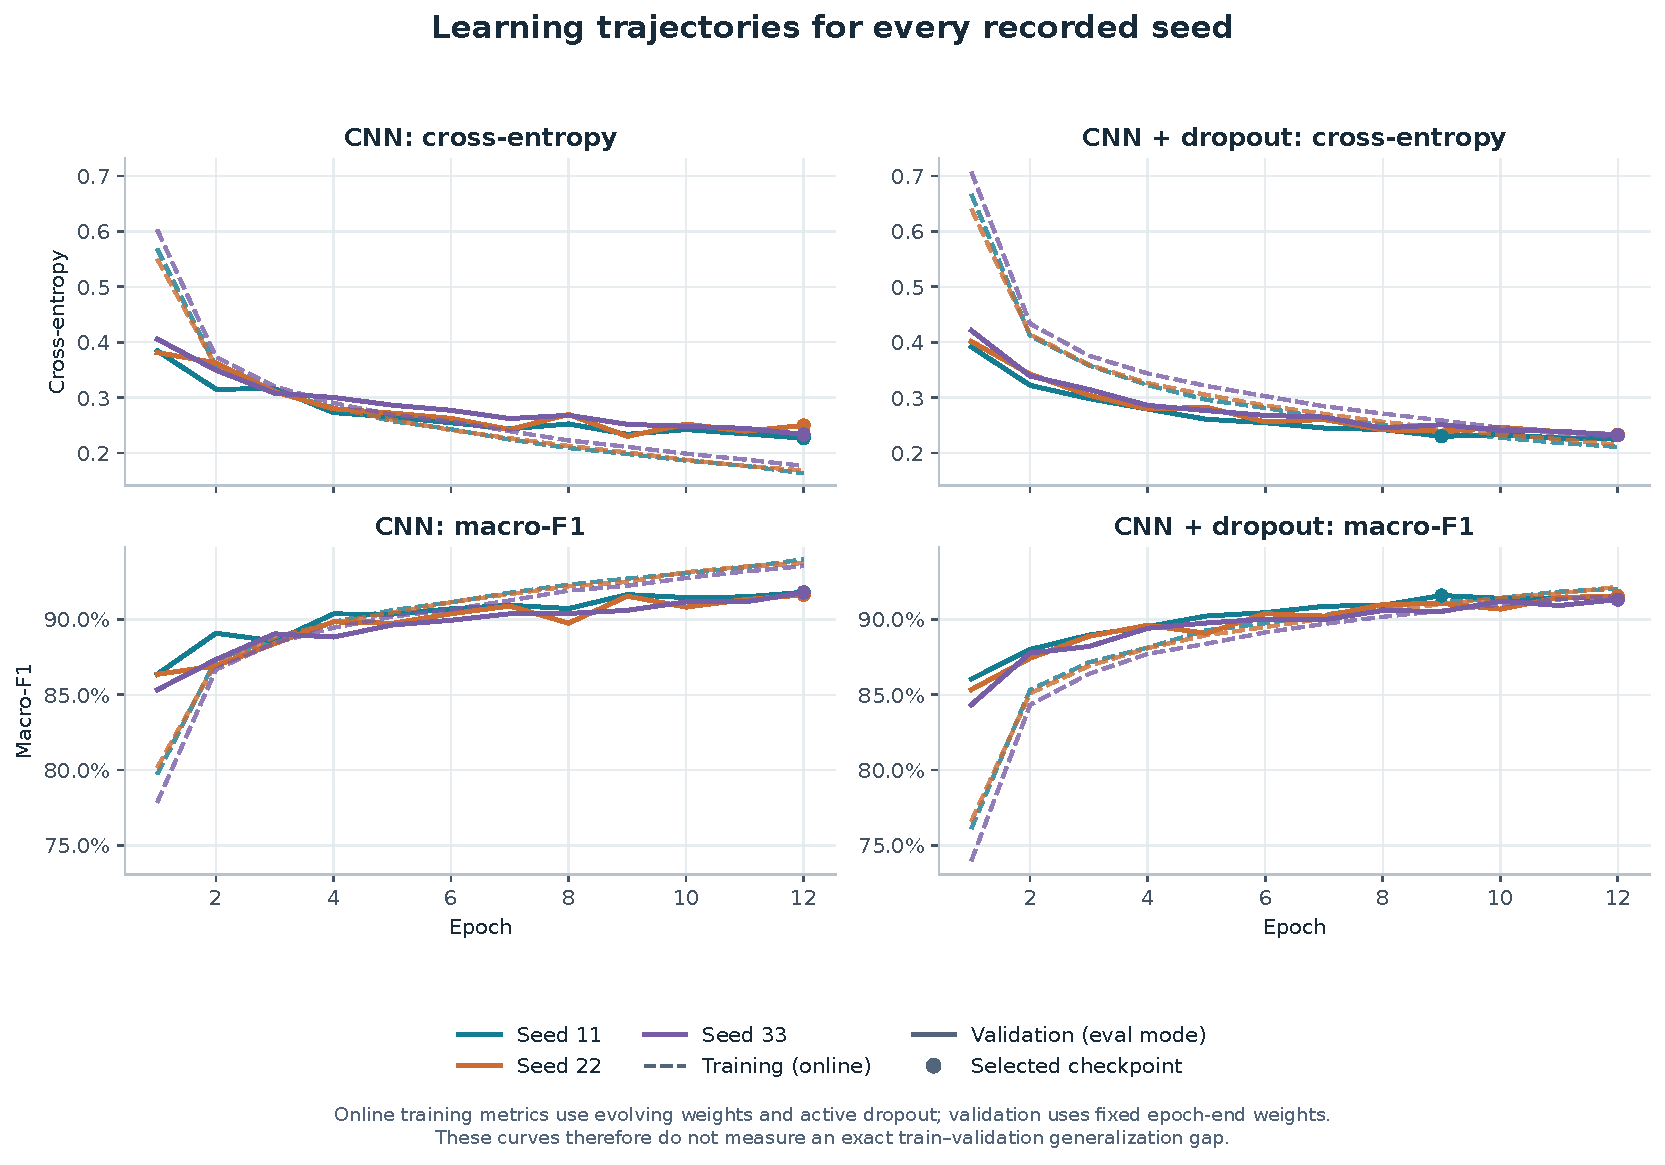
\includegraphics[width=\textwidth]{learning_curves.pdf}
\caption{Learning curves for all six runs. Dashed training curves aggregate minibatch predictions from evolving weights, with dropout active where applicable. Solid validation curves use fixed epoch-end weights in evaluation mode. The difference between these curves is therefore not an exact like-for-like generalization gap. Dots mark checkpoints selected by validation macro-F1.}
\label{fig:curves}
\end{figure*}

Dropout yields higher online training loss and lower online training F1 at the end of training, consistent with a harder stochastic training objective. Its validation loss can be competitive even when its validation or test macro-F1 is lower: cross-entropy scores probability assignments, whereas macro-F1 depends on discrete predictions and the distribution of errors across classes. Neither the curve gap nor a lower loss alone establishes that dropout improves the chosen target metric.

The CNN tuning budget is one prescribed hyperparameter setting per variant, repeated with three seeds: six fits and 72 total training epochs. No learning-rate or dropout-rate search is conducted. Baseline tuning uses three $C$ values. The final baseline grid takes \BaselineBudget\ seconds; including the initial convergence-repair attempt, observed baseline fitting totals \BaselineAllBudget\ seconds. The selected baseline fit takes \LogTime\ seconds. CNN fitting plus validation totals \TotalCNNTime\ seconds across all runs; mean per-run times are shown in Table~\ref{tab:runs}. These times exclude dataset loading, the sanity fit, plotting, and final test verification.

Runs use an Apple M4 CPU on macOS 26.5.2 (arm64), with ten logical CPUs, 16 GiB RAM, and four PyTorch/BLAS threads. MPS is available but unused; CUDA is unavailable. The recorded environment is Python 3.14.2, PyTorch 2.15.0, scikit-learn 1.9.1, NumPy 2.5.5, pandas 3.1.1, and Matplotlib 3.11.2. The complete dependency file is included. Wall times reflect this machine and background load, not a standardized speed benchmark; the variant order was not randomized.

\section{Exploratory Error Analysis}
\subsection{Which categories remain difficult?}
Table~\ref{tab:classes} shows class F1, averaged across all three seeds for each neural variant. Shirt is the least accurate category by F1 in every model family: 59.55\% for logistic regression, 73.50\% for the plain CNN, and 72.15\% for dropout. Coats, pullovers, and T-shirts are the next low-performing neural categories. Trousers, bags, and footwear are generally easier. Dropout's class-level changes are not uniformly negative: for example, sandal F1 increases, while shirt F1 decreases. Macro-F1 aggregates those gains and losses.

\begin{table}[t]
\caption{Label mapping and per-class test F1 (\%). Neural columns are means of three runs; the baseline is one fit. Class difficulty is exploratory.}
\label{tab:classes}
\centering
\begin{tabular}{rlrrr}
\toprule ID & Category & Logistic & CNN & Dropout \\
\midrule
\csname @@input\endcsname generated/class_rows.tex 
\bottomrule
\end{tabular}
\end{table}

Seed 11 was designated in the notebook before test evaluation for illustrative matrices and images. It is not the best test run selected afterward. Figure~\ref{fig:confusion} shows its dropout confusion matrix. Of the 1,000 true shirts, 142 are labeled T-shirt/top, 73 coat, and 61 pullover. In the reverse direction, 74 T-shirts are called shirts. The model also confuses 68 coats with pullovers and 53 pullovers with coats. These are specific garment confusions rather than a generic statement that ``similar classes'' fail.

The pattern is not confined to one seed. Across plain CNN runs, the mean number of shirts predicted as T-shirts is 131; across dropout runs it is 134. Mean shirt-to-coat errors are 78.33 and 83.33, respectively. All seven count matrices and the full directed error-pair table are saved. Per-seed counts should not be treated as independent measurements of new test populations: each run sees the same images.



\subsection{What is visible in representative mistakes?}
Figure~\ref{fig:errors} selects the lowest official test index from each of the four most frequent directed confusion pairs in the seed-11 dropout run. This deterministic rule emphasizes common failures, not the prevalence of particular visual appearances. It was applied after test evaluation; the following explanations are exploratory hypotheses rather than verified causes.

Image 40, a shirt predicted as T-shirt/top, has a short-sleeved outline. Small dark marks down the center suggest a fastening detail, but occupy few pixels. Image 381, a T-shirt/top predicted as shirt, has a wide neckline and loose sleeves; its coarse outline resembles another upper-body garment. Image 117, a shirt predicted as coat, has long sleeves, a long torso, and vertical central structure. Image 25, a coat predicted as pullover, is dark with low-contrast central details. The supplementary eight-image plot in the notebook includes additional shirt, pullover, and coat mistakes.

These observations make ambiguity at $28\times28$ resolution a plausible explanation. They do not demonstrate that the network attended to these particular features: no attribution or counterfactual intervention was performed. The labels are retained as supplied. A future study could examine higher-resolution data or explicit local-detail representations, but those changes would require a new validation protocol rather than tuning against these inspected test mistakes.

\begin{figure*}[t]
\begin{minipage}[t]{0.48\textwidth}
\centering
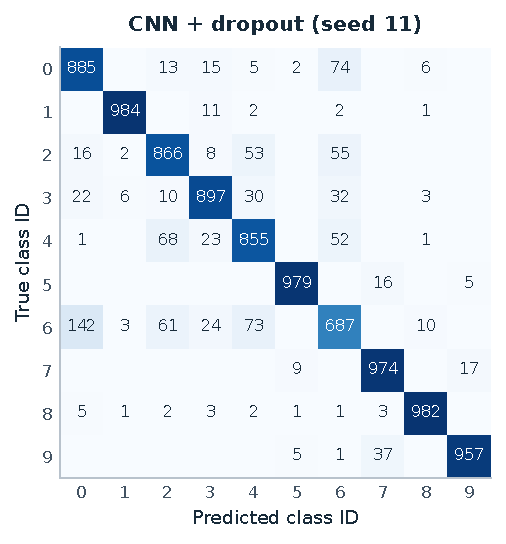
\includegraphics[width=\linewidth,height=3.05in,keepaspectratio]{confusion_dropout_11.pdf}
\caption{Dropout CNN, predeclared illustrative seed 11. Rows are true labels and columns predicted labels; integer entries are counts. Each row has 1,000 test images. Label mapping: Table~\ref{tab:classes}.}
\label{fig:confusion}
\end{minipage}\hfill
\begin{minipage}[t]{0.48\textwidth}
\centering
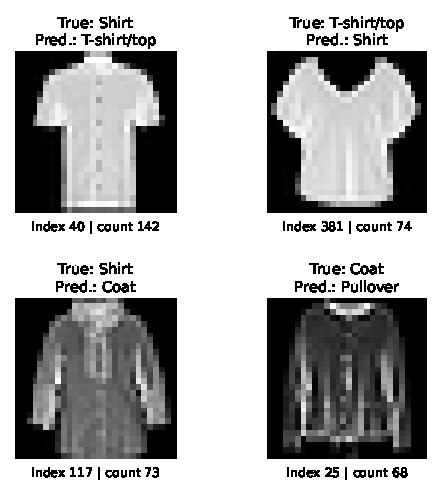
\includegraphics[width=\linewidth,height=3.05in,keepaspectratio]{generated/errors_grid.pdf}
\caption{Exploratory errors from the same model: first test index in each of its four most frequent directed confusion pairs. Supplied/predicted labels are shown. Nearest-neighbor enlargement preserves pixel structure.}
\label{fig:errors}
\end{minipage}
\end{figure*}

\section{Discussion and Limitations}
The primary finding is that head dropout at the chosen rate does not improve held-out macro-F1 within this architecture and 12-epoch procedure. One plausible explanation is that 48,000 training examples already constrain the small network sufficiently, so the added regularization costs more fitting ability than it gains in generalization. Another is that dropout needs a different training duration or learning rate to realize a benefit. Those possibilities are interpretations, not tested alternatives. The experiment intentionally holds those factors fixed to answer the stated question.

Several limits bound the conclusion. First, one split, one model width, one dropout location/rate, and three training seeds do not establish a universal effect of dropout. The unusually small plain-CNN seed SD is a property of these observed runs and should not be assumed elsewhere. No confidence interval or significance claim is attached to the mean effect. Second, the test set is reused across seeds, and the audit cannot detect every latent product dependency or near duplicate. Third, grayscale catalog thumbnails omit color, texture detail, clutter, and acquisition shifts common in real applications. There is no demographic annotation or deployment evaluation from which to infer fairness or real-camera performance.

Fourth, fixed epochs equalize the number of optimization passes, not necessarily the amount of computation or the distance to convergence. Reported timings are descriptive. Fifth, the baseline grid is deliberately small; alternative classical features or larger searches might improve it. Finally, post-test image inspection provides useful error descriptions but cannot establish mechanisms. The absence of a dropout benefit here is informative precisely because it is reported without changing the procedure until a positive outcome appears.

\section{Reproducibility and Verification}
The source notebook is the experiment entry point. A fresh-kernel execution using the README command, \texttt{python scripts/run\_notebook.py -{}-mode train}, completed all eight code cells with zero error outputs and retained 96 visible outputs. It includes the pre-run hypothesis, data audit, checks, baseline search, six CNN fits, freeze, evaluation, and analysis. The entry point explicitly launches the current Python interpreter as its kernel, avoiding dependence on an unrelated global kernelspec.

The code package contains exact dependency versions, configuration and seeds, original split indices, per-epoch histories, timing/selection records, all seven checkpoints, official-test indices and predictions, numerical summaries, and report sources. The verification routine independently recomputes accuracy, macro-F1, and balanced accuracy from the saved predictions and matches the comparison table to tolerance $10^{-12}$. It also reloads every checkpoint and confirms identical predictions on all 10,000 test examples. A separate verify mode replays the supplied evidence without claiming a second training replication. The frozen manifest protects experiment provenance; plotting and document assembly do not fit models.

The implementation was written for this study with AI assistance. It uses standard PyTorch layers, optimizer, and loss functions, and scikit-learn's estimator and metrics; it does not import pretrained weights or external training examples. The local training loop follows the documented optimization pattern~\cite{pytorch}, and the dataset, regularization rationale, and library sources are cited. The report uses the unmodified IEEEtran conference class~\cite{ieeetran}.

\section{Conclusion}
For this fixed Fashion-MNIST study, adding $p=0.30$ head dropout decreases mean test macro-F1 from \PlainFone\% to \DropFone\%, a change of \MeanDelta\ percentage points. All three matched-seed differences are negative. The original improvement hypothesis is unsupported, while both CNNs substantially exceed the logistic baseline. Shirts remain the hardest category; shirt/T-shirt and shirt/coat/pullover confusions dominate the exploratory analysis. Broader claims require additional experiments and untouched evaluation data.

\section*{Contribution and Review Statement}
Actual team names and individual contributions are pending insertion by the team. The team reported reviewing the existing work; review of the final generated report, notebook, slides, and recording remains to be confirmed. AI assistance is disclosed above. Each member must verify the final materials and accurately describe their own contribution before submission.

\clearpage
\begin{thebibliography}{9}
\bibitem{fashion} H. Xiao, K. Rasul, and R. Vollgraf, ``Fashion-MNIST: a novel image dataset for benchmarking machine learning algorithms,'' arXiv:1708.07747v2, 2017. [Online]. Available: \url{https://arxiv.org/abs/1708.07747v2}
\bibitem{dataset} Zalando Research, ``Fashion-MNIST: original data and label mapping,'' GitHub repository. [Online]. Available: \url{https://github.com/zalandoresearch/fashion-mnist}. Accessed: Nov. 20, 2026.
\bibitem{dropout} N. Srivastava, G. Hinton, A. Krizhevsky, I. Sutskever, and R. Salakhutdinov, ``Dropout: a simple way to prevent neural networks from overfitting,'' \emph{Journal of Machine Learning Research}, vol. 15, no. 56, pp. 1929--1958, 2014. [Online]. Available: \url{https://jmlr.org/papers/v15/srivastava14a.html}
\bibitem{sklearn} Scikit-learn developers, ``LogisticRegression,'' scikit-learn 1.9.1 documentation. [Online]. Available: \url{https://scikit-learn.org/stable/modules/generated/sklearn.linear_model.LogisticRegression.html}. Accessed: Nov. 20, 2026.
\bibitem{pytorch} PyTorch contributors, ``Optimizing model parameters,'' \emph{Learn the Basics}, PyTorch 2.15.0 documentation. [Online]. Available: \url{https://docs.pytorch.org/tutorials/beginner/basics/optimization_tutorial.html}. Accessed: Nov. 20, 2026.
\bibitem{ieeetran} M. Shell, ``IEEEtran: document class for IEEE Transactions journals and conferences,'' version 1.8b, 2015. [Online]. Available: \url{https://ctan.org/pkg/ieeetran}. Accessed: Nov. 20, 2026.
\end{thebibliography}
\end{document}
